\item \textbf{{[}HCI/PRELIM/9569/2021/P1/Q8{]}}

The school is designing a website to allow ordering of meal. The database
stores data about 
\begin{itemize}
\item students 
\item meal information
\item order information 
\end{itemize}
An order contains one meal only. 

Each meal can be purchased by different students. 

A student never places more than one meal on any day. 

The data is stored in a relational database. 
\begin{center}
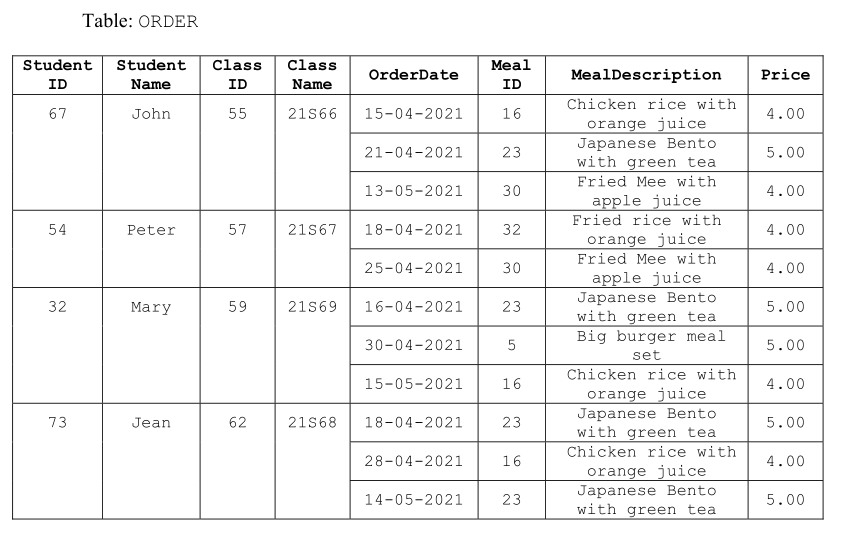
\includegraphics[width=0.5\paperwidth]{C:/Users/Admin/Desktop/Github/question_bank/LyX/static/img/9569-HCI-2021-P1-Q8-1}
\par\end{center}
\begin{enumerate}
\item Explain why the table is not in first normal form (1NF). \hfill{}{[}1{]}
\end{enumerate}
The following is an attempt to reduce data redundancy:
\begin{center}
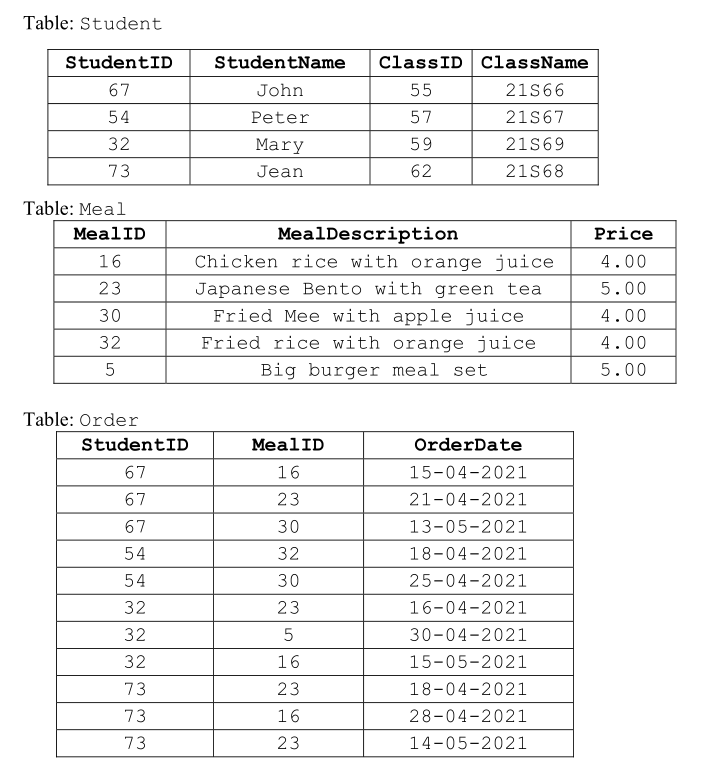
\includegraphics[width=0.5\paperwidth]{C:/Users/Admin/Desktop/Github/question_bank/LyX/static/img/9569-HCI-2021-P1-Q8-2}
\par\end{center}
\begin{enumerate}
\item[(b)]  State suitable primary key(s) for each table.\hfill{} {[}3{]}
\item[(c)]  Explain the reasons for reducing data redundancy in a relational
database. \hfill{}{[}2{]}
\item[(d)]  Draw an entity-relationship (E-R) diagram showing the degree of
the relations. \hfill{}{[}2{]}
\item[(e)]  State which table is not in third normal form (3NF) and explain
why. {[}2{]} 
\end{enumerate}
A table description can be expressed as: 
\noindent \begin{center}
\texttt{TableName (}\texttt{\uline{Attribute1}}\texttt{, Attribute2{*},
Attribute3, \dots ) }
\par\end{center}

The primary key is indicated by underlining one or more attributes.
Foreign keys are indicated by using a dashed underline/asterisk.
\begin{enumerate}
\item[(f)]  Write table descriptions for the required tables in the databases
so they are in third normal form (3NF). \hfill{}{[}4{]}
\item[(g)]  Write an SQL query to output the student names and date of order
of all the orders for the meal \textquotedblleft \texttt{Japanese
Bento with green tea}\textquotedblright .\hfill{} {[}3{]}
\end{enumerate}